\subsection*{User stories for energy forecasting for offshore wind parks using wind lidar}

\begin{table*}[!h]
 \centering
 \caption{Actors in energy forecasting for offshore wind farms today}
 % set up banded rows for the agenda and add lines to the columns
 \arrayrulecolor{Task32Blue2!15}
 \rowcolors{2}{Task32Blue2!5}{white}
 \begin{tabular}{@{}|p{0.125\textwidth}|p{0.255\textwidth}|p{0.255\textwidth}|p{0.255\textwidth}|@{}}
 \rowcolor{Task32Blue2} & \textbf{Alice} & \textbf{Bob} & \textbf{Chris}  \\
They are: & 
    Wind farm operator & 
    Forecaster & 
    Energy trader \\
Their biggest problem is: & 
    Unknown wind conditions in the future & 
    No data & 
    If they cannot deliver sold energy \\
Success for them is: & 
    Wants to sell her energy & 
    Having low uncertainty forecast & 
    Highest revenue \\
Problem statement: & 
    \multicolumn{3}{|p{0.765\textwidth+4\tabcolsep+2\arrayrulewidth}|}{We need the best wind data to produce a low-uncertainty energy yield forecast}\\
\end{tabular}
\label{tab:02_offshoreforecasting_now}
\end{table*}


\begin{figure*}[!h]
    \centering
    \fbox{
    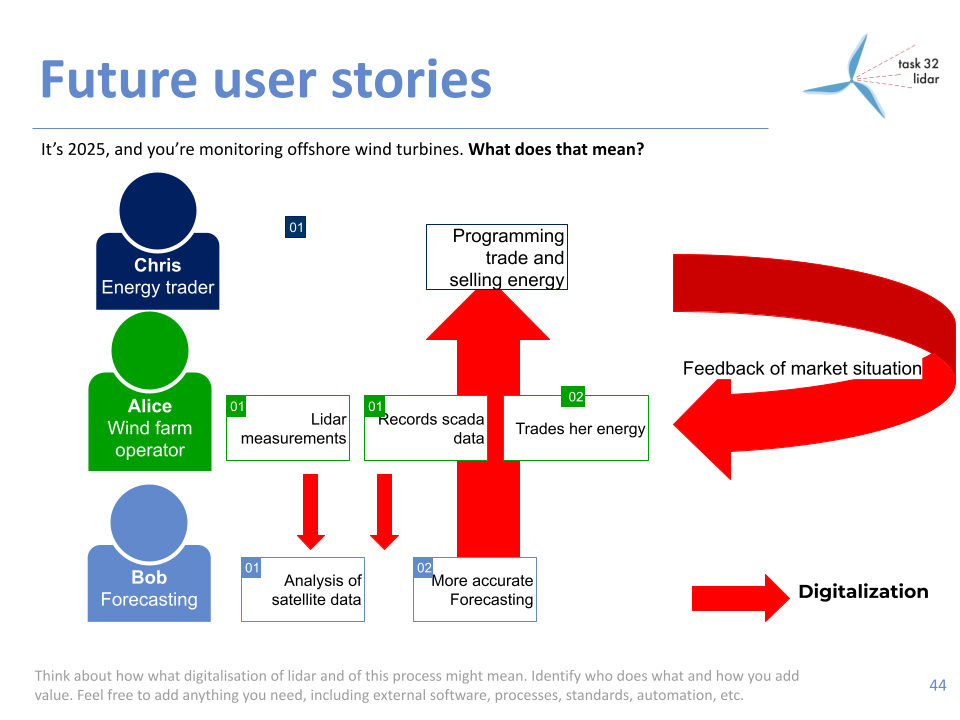
\includegraphics[width=0.85\textwidth]{figures/02_offshoreforecasting.png}
    }
    \caption{A vision for future energy trading for offshore wind}
    \label{fig:02_offshoreforecasting_future}
\end{figure*}
